\noindent
\includegraphics[height=1.25cm]{images/pictograms/replication}
\includegraphics[height=1.25cm]{images/pictograms/benchmark}
\includegraphics[height=1.25cm]{images/pictograms/under_construction}
\includegraphics[height=1.25cm]{images/pictograms/FDM}
\includegraphics[height=1.25cm]{images/pictograms/temperature}
\includegraphics[height=1.25cm]{images/pictograms/paraview}

%%%%%%%%%%%%%%%%%%%%%%%%%%%%%%%%%%%%%%%%%%%%%%%%%%%%%%%%%%%%%%%%%%%%%%%%%%%%%%%%%%%%%%%%%%%%%%%%%%%

\begin{flushright} {\tiny {\color{gray} python\_codes/fieldstone\_158/text.tex}} \end{flushright}

%\lstinputlisting[language=bash,basicstyle=\small]{python_codes/template_keywords.key}

\par\noindent\rule{\textwidth}{0.4pt}

\begin{center}
\infortran
{\small Code: \url{https://github.com/cedrict/fieldstone/tree/master/python_codes/fieldstone_158}}
\end{center}

\par\noindent\rule{\textwidth}{0.4pt}


%%%%%%%%%%%%%%%%%%%%%%%%%%%%%%%%%%%%%%%%%%%%%%%%%%%%%%%%%%%%%%%%%%%%%%%%%%%%%%%%%%%%%%%%%%%%%%%%%%%


\begin{center}
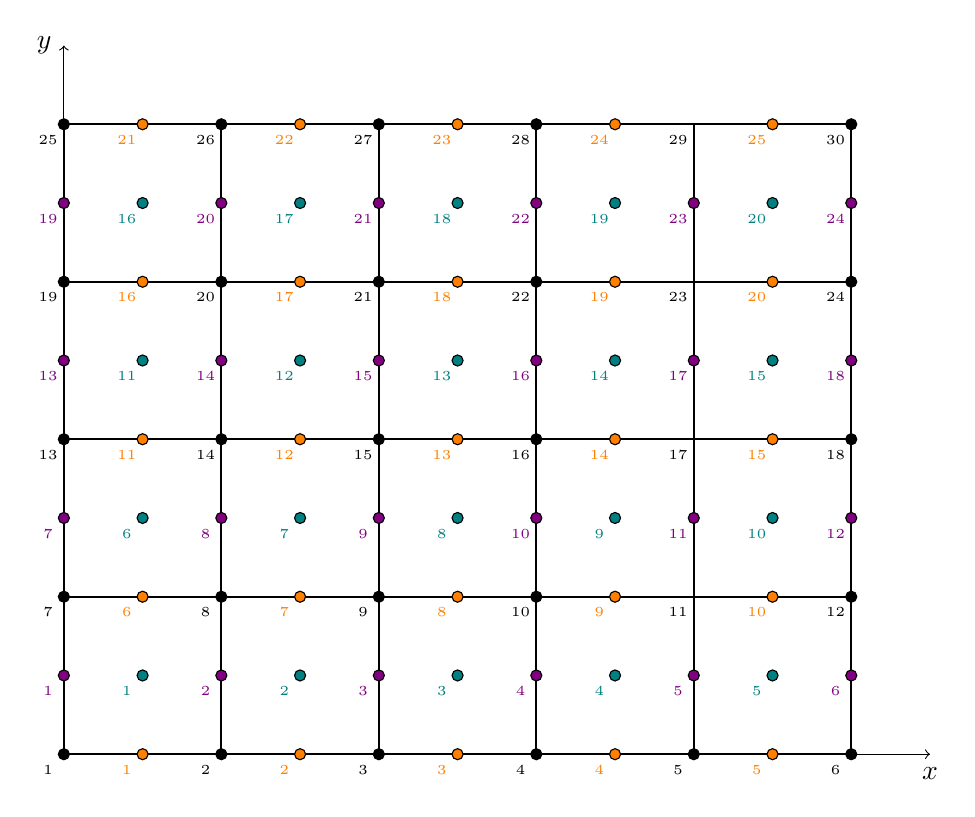
\begin{tikzpicture}
%\draw[fill=gray!23,gray!23](0,0) rectangle (12,10);
%\draw[step=0.5cm,gray,very thin] (0,0) grid (12,10); %background grid

\draw[thick] (0,0) -- (10,0) -- (10,8) -- (0,8) -- cycle ; %1-4
\draw[thick] (0,2) -- (10,2)  ; 
\draw[thick] (0,4) -- (10,4)  ; 
\draw[thick] (0,6) -- (10,6)  ; 
\draw[thick] (2,0) -- (2,8)  ; 
\draw[thick] (4,0) -- (4,8)  ; 
\draw[thick] (6,0) -- (6,8)  ; 
\draw[thick] (8,0) -- (8,8)  ; 

%pressure nodes
\draw[black,fill=teal] (1,1)   circle (2pt); %1
\draw[black,fill=teal] (3,1)   circle (2pt); %1
\draw[black,fill=teal] (5,1)   circle (2pt); %1
\draw[black,fill=teal] (7,1)   circle (2pt); %1
\draw[black,fill=teal] (9,1)   circle (2pt); %1
\draw[black,fill=teal] (1,3)   circle (2pt); %1
\draw[black,fill=teal] (3,3)   circle (2pt); %1
\draw[black,fill=teal] (5,3)   circle (2pt); %1
\draw[black,fill=teal] (7,3)   circle (2pt); %1
\draw[black,fill=teal] (9,3)   circle (2pt); %1
\draw[black,fill=teal] (1,5)   circle (2pt); %1
\draw[black,fill=teal] (3,5)   circle (2pt); %1
\draw[black,fill=teal] (5,5)   circle (2pt); %1
\draw[black,fill=teal] (7,5)   circle (2pt); %1
\draw[black,fill=teal] (9,5)   circle (2pt); %1
\draw[black,fill=teal] (1,7)   circle (2pt); %1
\draw[black,fill=teal] (3,7)   circle (2pt); %1
\draw[black,fill=teal] (5,7)   circle (2pt); %1
\draw[black,fill=teal] (7,7)   circle (2pt); %1
\draw[black,fill=teal] (9,7)   circle (2pt); %1
\node[] at (0.8,0.8) {\tiny \color{teal} 1};
\node[] at (2.8,0.8) {\tiny \color{teal} 2};
\node[] at (4.8,0.8) {\tiny \color{teal} 3};
\node[] at (6.8,0.8) {\tiny \color{teal} 4};
\node[] at (8.8,0.8) {\tiny \color{teal} 5};
\node[] at (0.8,2.8) {\tiny \color{teal} 6};
\node[] at (2.8,2.8) {\tiny \color{teal} 7};
\node[] at (4.8,2.8) {\tiny \color{teal} 8};
\node[] at (6.8,2.8) {\tiny \color{teal} 9};
\node[] at (8.8,2.8) {\tiny \color{teal} 10};
\node[] at (0.8,4.8) {\tiny \color{teal} 11};
\node[] at (2.8,4.8) {\tiny \color{teal} 12};
\node[] at (4.8,4.8) {\tiny \color{teal} 13};
\node[] at (6.8,4.8) {\tiny \color{teal} 14};
\node[] at (8.8,4.8) {\tiny \color{teal} 15};
\node[] at (0.8,6.8) {\tiny \color{teal} 16};
\node[] at (2.8,6.8) {\tiny \color{teal} 17};
\node[] at (4.8,6.8) {\tiny \color{teal} 18};
\node[] at (6.8,6.8) {\tiny \color{teal} 19};
\node[] at (8.8,6.8) {\tiny \color{teal} 20};

% u nodes
\draw[black,fill=violet] (0,1)   circle (2pt); 
\draw[black,fill=violet] (2,1)   circle (2pt); 
\draw[black,fill=violet] (4,1)   circle (2pt); 
\draw[black,fill=violet] (6,1)   circle (2pt); 
\draw[black,fill=violet] (8,1)   circle (2pt); 
\draw[black,fill=violet] (10,1)   circle (2pt);

\draw[black,fill=violet] (0,3)   circle (2pt); 
\draw[black,fill=violet] (2,3)   circle (2pt); 
\draw[black,fill=violet] (4,3)   circle (2pt); 
\draw[black,fill=violet] (6,3)   circle (2pt); 
\draw[black,fill=violet] (8,3)   circle (2pt); 
\draw[black,fill=violet] (10,3)   circle (2pt);

\draw[black,fill=violet] (0,5)   circle (2pt); 
\draw[black,fill=violet] (2,5)   circle (2pt); 
\draw[black,fill=violet] (4,5)   circle (2pt); 
\draw[black,fill=violet] (6,5)   circle (2pt); 
\draw[black,fill=violet] (8,5)   circle (2pt); 
\draw[black,fill=violet] (10,5)   circle (2pt);

\draw[black,fill=violet] (0,7)   circle (2pt); 
\draw[black,fill=violet] (2,7)   circle (2pt); 
\draw[black,fill=violet] (4,7)   circle (2pt); 
\draw[black,fill=violet] (6,7)   circle (2pt); 
\draw[black,fill=violet] (8,7)   circle (2pt); 
\draw[black,fill=violet] (10,7)   circle (2pt);

\node[] at (-0.2,0.8) {\tiny \color{violet} 1};
\node[] at (1.8,0.8) {\tiny \color{violet} 2};
\node[] at (3.8,0.8) {\tiny \color{violet} 3};
\node[] at (5.8,0.8) {\tiny \color{violet} 4};
\node[] at (7.8,0.8) {\tiny \color{violet} 5};
\node[] at (9.8,0.8) {\tiny \color{violet} 6};

\node[] at (-0.2,2.8) {\tiny \color{violet} 7};
\node[] at (1.8,2.8) {\tiny \color{violet} 8};
\node[] at (3.8,2.8) {\tiny \color{violet} 9};
\node[] at (5.8,2.8) {\tiny \color{violet} 10};
\node[] at (7.8,2.8) {\tiny \color{violet} 11};
\node[] at (9.8,2.8) {\tiny \color{violet} 12};

\node[] at (-0.2,4.8) {\tiny \color{violet} 13};
\node[] at (1.8,4.8) {\tiny \color{violet} 14};
\node[] at (3.8,4.8) {\tiny \color{violet} 15};
\node[] at (5.8,4.8) {\tiny \color{violet} 16};
\node[] at (7.8,4.8) {\tiny \color{violet} 17};
\node[] at (9.8,4.8) {\tiny \color{violet} 18};

\node[] at (-0.2,6.8) {\tiny \color{violet} 19};
\node[] at (1.8,6.8) {\tiny \color{violet} 20};
\node[] at (3.8,6.8) {\tiny \color{violet} 21};
\node[] at (5.8,6.8) {\tiny \color{violet} 22};
\node[] at (7.8,6.8) {\tiny \color{violet} 23};
\node[] at (9.8,6.8) {\tiny \color{violet} 24};

% v nodes
\draw[black,fill=orange] (1,0)   circle (2pt); 
\draw[black,fill=orange] (3,0)   circle (2pt); 
\draw[black,fill=orange] (5,0)   circle (2pt); 
\draw[black,fill=orange] (7,0)   circle (2pt); 
\draw[black,fill=orange] (9,0)   circle (2pt); 

\draw[black,fill=orange] (1,2)   circle (2pt); 
\draw[black,fill=orange] (3,2)   circle (2pt); 
\draw[black,fill=orange] (5,2)   circle (2pt); 
\draw[black,fill=orange] (7,2)   circle (2pt); 
\draw[black,fill=orange] (9,2)   circle (2pt); 

\draw[black,fill=orange] (1,4)   circle (2pt); 
\draw[black,fill=orange] (3,4)   circle (2pt); 
\draw[black,fill=orange] (5,4)   circle (2pt); 
\draw[black,fill=orange] (7,4)   circle (2pt); 
\draw[black,fill=orange] (9,4)   circle (2pt); 

\draw[black,fill=orange] (1,6)   circle (2pt); 
\draw[black,fill=orange] (3,6)   circle (2pt); 
\draw[black,fill=orange] (5,6)   circle (2pt); 
\draw[black,fill=orange] (7,6)   circle (2pt); 
\draw[black,fill=orange] (9,6)   circle (2pt); 

\draw[black,fill=orange] (1,8)   circle (2pt); 
\draw[black,fill=orange] (3,8)   circle (2pt); 
\draw[black,fill=orange] (5,8)   circle (2pt); 
\draw[black,fill=orange] (7,8)   circle (2pt); 
\draw[black,fill=orange] (9,8)   circle (2pt); 

\node[] at (0.8,-0.2) {\tiny \color{orange} 1};
\node[] at (2.8,-0.2) {\tiny \color{orange} 2};
\node[] at (4.8,-0.2) {\tiny \color{orange} 3};
\node[] at (6.8,-0.2) {\tiny \color{orange} 4};
\node[] at (8.8,-0.2) {\tiny \color{orange} 5};

\node[] at (0.8,1.8) {\tiny \color{orange} 6};
\node[] at (2.8,1.8) {\tiny \color{orange} 7};
\node[] at (4.8,1.8) {\tiny \color{orange} 8};
\node[] at (6.8,1.8) {\tiny \color{orange} 9};
\node[] at (8.8,1.8) {\tiny \color{orange} 10};

\node[] at (0.8,3.8) {\tiny \color{orange} 11};
\node[] at (2.8,3.8) {\tiny \color{orange} 12};
\node[] at (4.8,3.8) {\tiny \color{orange} 13};
\node[] at (6.8,3.8) {\tiny \color{orange} 14};
\node[] at (8.8,3.8) {\tiny \color{orange} 15};

\node[] at (0.8,5.8) {\tiny \color{orange} 16};
\node[] at (2.8,5.8) {\tiny \color{orange} 17};
\node[] at (4.8,5.8) {\tiny \color{orange} 18};
\node[] at (6.8,5.8) {\tiny \color{orange} 19};
\node[] at (8.8,5.8) {\tiny \color{orange} 20};

\node[] at (0.8,7.8) {\tiny \color{orange} 21};
\node[] at (2.8,7.8) {\tiny \color{orange} 22};
\node[] at (4.8,7.8) {\tiny \color{orange} 23};
\node[] at (6.8,7.8) {\tiny \color{orange} 24};
\node[] at (8.8,7.8) {\tiny \color{orange} 25};

%------------------------------------------------

\draw[black,fill=black] (0,0)   circle (2pt); 
\draw[black,fill=black] (2,0)   circle (2pt); 
\draw[black,fill=black] (4,0)   circle (2pt); 
\draw[black,fill=black] (6,0)   circle (2pt); 
\draw[black,fill=black] (8,0)   circle (2pt); 
\draw[black,fill=black] (10,0)   circle (2pt); 

\draw[black,fill=black] (0,2)   circle (2pt); 
\draw[black,fill=black] (2,2)   circle (2pt); 
\draw[black,fill=black] (4,2)   circle (2pt); 
\draw[black,fill=black] (6,2)   circle (2pt); 
\draw[black,fill=black] (10,2)   circle (2pt); 

\draw[black,fill=black] (0,4)   circle (2pt); 
\draw[black,fill=black] (2,4)   circle (2pt); 
\draw[black,fill=black] (4,4)   circle (2pt); 
\draw[black,fill=black] (6,4)   circle (2pt); 
\draw[black,fill=black] (10,4)   circle (2pt); 

\draw[black,fill=black] (0,6)   circle (2pt); 
\draw[black,fill=black] (2,6)   circle (2pt); 
\draw[black,fill=black] (4,6)   circle (2pt); 
\draw[black,fill=black] (6,6)   circle (2pt); 
\draw[black,fill=black] (10,6)   circle (2pt); 

\draw[black,fill=black] (0,8)   circle (2pt); 
\draw[black,fill=black] (2,8)   circle (2pt); 
\draw[black,fill=black] (4,8)   circle (2pt); 
\draw[black,fill=black] (6,8)   circle (2pt); 
\draw[black,fill=black] (10,8)   circle (2pt); 


\node[] at (-0.2,-0.2) {\tiny 1};
\node[] at (1.8,-0.2) {\tiny 2};
\node[] at (3.8,-0.2) {\tiny 3};
\node[] at (5.8,-0.2) {\tiny 4};
\node[] at (7.8,-0.2) {\tiny 5};
\node[] at (9.8,-0.2) {\tiny 6};

\node[] at (-0.2,1.8) {\tiny 7};
\node[] at (1.8,1.8) {\tiny 8};
\node[] at (3.8,1.8) {\tiny 9};
\node[] at (5.8,1.8) {\tiny 10};
\node[] at (7.8,1.8) {\tiny 11};
\node[] at (9.8,1.8) {\tiny 12};

\node[] at (-0.2,3.8) {\tiny 13};
\node[] at (1.8,3.8) {\tiny 14};
\node[] at (3.8,3.8) {\tiny 15};
\node[] at (5.8,3.8) {\tiny 16};
\node[] at (7.8,3.8) {\tiny 17};
\node[] at (9.8,3.8) {\tiny 18};

\node[] at (-0.2,5.8) {\tiny 19};
\node[] at (1.8,5.8) {\tiny 20};
\node[] at (3.8,5.8) {\tiny 21};
\node[] at (5.8,5.8) {\tiny 22};
\node[] at (7.8,5.8) {\tiny 23};
\node[] at (9.8,5.8) {\tiny 24};

\node[] at (-0.2,7.8) {\tiny 25};
\node[] at (1.8,7.8) {\tiny 26};
\node[] at (3.8,7.8) {\tiny 27};
\node[] at (5.8,7.8) {\tiny 28};
\node[] at (7.8,7.8) {\tiny 29};
\node[] at (9.8,7.8) {\tiny 30};

%-------------------------------------------------

\draw[thin,->] (10,0) -- (11,0); %x
\node[] at (11,-0.25) {$x$};
\draw[thin,->] (0,8) -- (0,9); %y
\node[] at (-0.25,9) {$y$};

\end{tikzpicture}
\end{center}

